\section{Zielsetzung}
\label{sec:Zielsetzung}
Die Funktionsweise eines Lock-In-Verstärkers soll erarbeitet werden.
\section{Theorie}
\label{sec:Theorie}

Der Lock-In-Verstärker ist ein nützliches Werkzeug in der Messtechnik, insbesondere bei der Messung sehr schwacher Signale in lauten Umgebungen. In Abbildung 1 ist der Schematische Aufbau skizziert. Er kann auch verwendet werden, um das Nutzsignal aus einem Meßsignal zu isolieren, das von zufälligen Störgrößen beeinflusst wird. Ein Beispiel hierfür wäre die Messung der Magnetisierung eines Materials in einem Magnetfeld, bei dem die magnetischen Störgrößen des Materials selbst zu Rauschen führen können. Der Lock-In-Verstärker kann in solchen Fällen das Nutzsignal isolieren und verstärken, um eine genauere Messung zu ermöglichen. \\
\\
Dies wird dadurch erreicht, dass das Meßsignal mit einem Referenzsignal multipliziert wird, das dieselbe Frequenz wie das Nutzsignal hat. Über den Phasenschieber kann die Phasenlage $\phi$ auf das Nutzsignal synchronisiert werden, sodass möglichst $\Delta \phi = 0$ gilt.
Durch die Multiplikation im Mischer entsteht ein Mischsignal, das die Phasenlage des Nutzsignals beibehält, aber die Amplitude der Rauschanteile verändert. Durch die Integration des Mischsignals über mehrere Perioden der Modulationsfrequenz werden sich die Beiträge der nicht zur Modulationsfrequenz synchronisierten Rauschbeiträge weitgehend aufheben, da sie sich bei der Multiplikation zufällig in ihrer Amplitude und Phase verändern. Nur die Beiträge, die mit der Modulationsfrequenz synchron sind, werden nach der Integration verstärkt. \\
Um die Empfindlichkeit des Lock-In-Verstärkers zu erhöhen, kann ein Tiefpassfilter nachgeschaltet werden, das die Bandbreite des Restrauschens reduziert. Dadurch werden nur die Nutzsignale in einem engen Frequenzbereich um die Modulationsfrequenz verstärkt, während Rauschsignale außerhalb dieses Bereichs unterdrückt werden.
In dem die Zeitkonstante $\tau = RC$ sehr groß gewählt wird, kann man die Bandbreite $\Delta v = \frac{1}{\pi RC}$ sehr klein machen, sodass nur Frequenzen nahe der gewünschten Frequenz
durchkommen. So können mit dem Lock-In-Verstärker erheblich bessere Ergebnisse als mit einem normalen Bandpass erreicht werden.\\
\\
\begin{figure}[H]
    \centering
    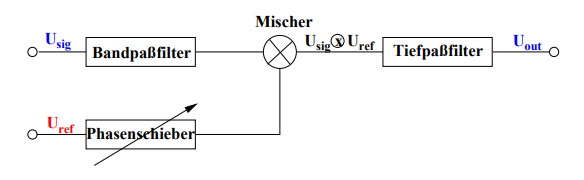
\includegraphics[width=0.8\textwidth]{img/abb1.png}
    \caption{Schematischer Aufbau eines Lock-In-Verstärkers\protect\footnotemark}
    \label{fig:abb1}
    \footnotetext{Entnommen aus V303: Der Lock-In-Verstärker \cite{V303}}
\end{figure}
Die Signalspannung ist gegeben durch
\begin{equation}
    U_{sig} = U_0 \cdot \sin(\omega t).
\end{equation}
Diese wird mit dem Referenzsignal $U_{ref}$ überlagert. Da als Referenzsignal ein Rechtecksignal der Amplitude 1 verwendet wird, kann es als folgende Fourierreihe
dargestellt werden
\begin{equation}\label{eqn:referenzFrequenz}
    U_{ref} = \frac{4}{\pi}\left(\sin{ωt} + \frac{1}{3}\sin{3ωt} + \frac{1}{5}\sin{5ωt} + \ldots\right).
\end{equation}
Das im Mischer entstehende Produkt aus Signal- und Referenzfrequenz ergibt sich dann zu
\begin{equation}\label{eqn:produkt}
    U_{sig} \times U_{ref} = \frac{2}{π}U_0\left( 1 - \frac{2}{3}\cos{2ωt} - \frac{2}{15}\cos{4ωt} - \frac{2}{35}\cos{6ωt} + \ldots\right).
\end{equation}
Im nachgeschalteten Tiefpassfilter werden die Signale über mehrere Perioden der Modulationsfrequenz integriert, sodass alle $\cos$ Terme wegfallen und man
\begin{equation}\label{eqn:U0}
    U_{out} = \frac{2}{\pi}\,U_0
\end{equation}
für die Ausgangsfrequenz erhält. Besteht zwischen Signal- und Referenzfrequenz einen Phasendifferenz $\Delta \phi$ so erhält man für die Ausgangsspannung
\begin{equation}\label{U0phi}
    U_{out} = \frac{2}{\pi}\,U_0\,\cos(\phi).
\end{equation}
Diese ist zwar proportional zu $U_0$, jedoch abhängig von der eingestellten Phase am Phasenschieber $\phi$.

\newpage